\documentclass[11pt,a4paper]{article}
\usepackage[T1]{fontenc}
\usepackage[utf8]{inputenc}
\usepackage{lmodern}
\usepackage{amsmath,amssymb}
\usepackage{booktabs}
\usepackage{graphicx}
\usepackage[margin=2.2cm]{geometry}
\usepackage[colorlinks=true,linkcolor=blue,citecolor=blue,urlcolor=blue]{hyperref}

\newcommand{\code}[1]{\texttt{#1}}

\title{Ten-day dry baroclinic wave with CGSEM and DGSEM\\[0.3em]
\large Resolution, time step, timing and accuracy on one GPU}
\author{CGDycore.jl}
\date{\today}

\begin{document}
\sloppy
\maketitle

\begin{abstract}
The dry baroclinic wave on the sphere is run for ten days with the
continuous Galerkin (CGSEM) and the discontinuous Galerkin (DGSEM)
spectral element dycores of CGDycore.jl. Both use their standard setup
for about 100~km horizontal resolution, the largest stable time step,
and Float32 and Float64. DGSEM is run with three pairs of numerical
fluxes: the vector-invariant form and two conservative forms. All runs use one NVIDIA
A100 on Levante and write no output. The day-10 surface pressure is
compared against a DGSEM run with twice the resolution in both
directions.
\end{abstract}

\section{Test case and setups}

The test is the dry baroclinic wave (\code{--Problem=BaroWaveDrySphere}):
flat ground, model top at 30~km, Earth radius and rotation, no damping
layer and no forcing, ten simulated days.

\paragraph{Standard setups (about 100 km).}
\begin{itemize}
\item \textbf{CGSEM}, job file \code{Jobs/NHSphere/CG/BaroWaveDrySphere\_32Elem}:
  cubed sphere with $n_\text{Panel}=32$ elements per panel edge,
  polynomial order $N=3$, 64 layers with exponential stretching
  (vertically linear elements, \code{OrdPolyZ=1}),
  vector-invariant momentum equation, shallow-atmosphere equations
  (\code{CompressibleShallow}), vertical upwinding,
  fourth-order hyperviscosity $5\cdot10^{14}\,\mathrm{m^4\,s^{-1}}$
  on curl, gradient and divergence.
  A second run uses the deep-atmosphere equations
  (\code{CompressibleDeep}), as DGSEM does.
\item \textbf{DGSEM}, job files \code{Jobs/NHSphere/DG/BaroWaveDrySphereDGQuad*}:
  cubed sphere with $n_\text{Panel}=20$, $N=4$; vertically 13 elements of
  order 4; deep-atmosphere equations with full Coriolis term; Cartesian
  velocity components; no explicit diffusion (dissipation only from the
  interface fluxes). Three flux pairs:
  \begin{itemize}
  \item \textbf{VI}: vector-invariant form, volume flux
    \code{VectorInvariant}, interface flux \code{RiemannVectorInvariant};
  \item \textbf{Cons}: conservative form, \code{KennedyGruberGrav} and
    \code{RiemannLMARS};
  \item \textbf{Diff}: conservative form, \code{KennedyGruberGravDiff} and
    \code{RiemannLMARSDiff} (pressure as a difference to a reference state).
  \end{itemize}
\end{itemize}

\paragraph{Additional CGSEM grids.} To separate the effect of the
polynomial order, CGSEM is also run with order 4:
\textbf{CG-A} with the DGSEM element grid ($n_\text{Panel}=20$, 52
uniform layers, i.e.\ the vertical node spacing of DGSEM) and
\textbf{CG-B} with about the same number of unknowns as DGSEM
($n_\text{Panel}=25$, 65 uniform layers). Both use the
deep-atmosphere equations and the deep Coriolis term, with
hyperviscosity $10^{15}$ (A) and $5\cdot10^{14}\,\mathrm{m^4\,s^{-1}}$ (B).

\paragraph{Reference.} DGSEM VI in Float64 with $n_\text{Panel}=40$,
$N=4$, 26 vertical elements of order 4, $\Delta t=42.5$~s.
Because the reference is itself a DGSEM VI run, the error measure
is a convergence measure for DGSEM. For CGSEM it also contains the
difference between the two discretizations.

\section{Resolution}

The horizontal spacing is given along a panel edge, which
spans $90^\circ$. CGSEM shares the element boundary nodes, so it has
$n_\text{Panel}N$ intervals per panel edge. DGSEM duplicates them, so
it has $n_\text{Panel}(N+1)$ nodes. The smallest node distance is the
first GLL gap: $0.276$ of the element width for $N=3$ and $0.173$ for
$N=4$. It is evaluated for the element at the panel centre on the
equator, with $1^\circ \approx 111.2$~km.

\begin{center}
\small
\begin{tabular}{lrrrrrrr}
\toprule
 & $n_\text{Panel}$ & $N$ & columns & vertical & mean $\Delta x$ & min $\Delta x$ & unknowns \\
 &  &  &  & nodes & & & per variable \\
\midrule
CGSEM standard & 32 & 3 & 55\,298 & 64 & $0.94^\circ$, 104 km & 86 km & 3.54\,M \\
CG-A           & 20 & 4 & 38\,402 & 52 & $1.13^\circ$, 125 km & 86 km & 2.00\,M \\
CG-B           & 25 & 4 & 60\,002 & 65 & $0.90^\circ$, 100 km & 69 km & 3.90\,M \\
DGSEM          & 20 & 4 & 60\,000 & $13\times5=65$ & $0.90^\circ$, 100 km & 86 km & 3.90\,M \\
DGSEM reference& 40 & 4 & 240\,000 & $26\times5=130$ & $0.45^\circ$, 50 km & 43 km & 31.2\,M \\
\bottomrule
\end{tabular}
\end{center}

Vertically, DGSEM has elements of $2.31$~km with 5 GLL nodes (mean node
spacing 577~m). CGSEM has 64 stretched layers (mean 469~m), CG-A 52
uniform layers (577~m) and CG-B 65 uniform layers (462~m).

\section{Time integration}

All runs use the same Rosenbrock W-method \code{SSP-Knoth}
(\code{--IntMethod=Rosenbrock}). It has three stages, and its explicit
part is the three-stage SSP Runge--Kutta method of Shu and Osher. The W-matrix
contains only the vertical (column) part of the Jacobian, the acoustic
and gravity terms, so the scheme is horizontally explicit and
vertically linearly implicit (HEVI). CGSEM solves the column systems
with \code{CGSEM.JacGPU!}. DGSEM uses \code{JacHEVI} with the default
\code{--HEVISolver=HDG}, a static condensation onto the element
interfaces of each column.

Since the horizontal terms are explicit, the time step is limited by
the horizontal Courant number $C=c\,\Delta t/\Delta x_\text{min}$, with
$c=340$~m/s and the smallest node distance from the table above.

\begin{center}
\small
\begin{tabular}{lrrl}
\toprule
 & $\Delta t$ [s] & $C$ & stability \\
\midrule
CGSEM standard & 150 & 0.59 & stable for 10 days \\
CGSEM standard & 230 & 0.90 & NaN after 0.11 days (value of the job file) \\
CG-A           & 150 & 0.59 & stable \\
CG-A           & 225 & 0.89 & NaN after 0.21 days \\
CG-B           & 120 & 0.59 & stable \\
DGSEM (all flux pairs) & 85 & 0.33 & stable \\
DGSEM reference& 42.5 & 0.33 & stable \\
\bottomrule
\end{tabular}
\end{center}

CGSEM is stable at $C=0.59$ and unstable at $C\approx0.9$. DGSEM is run
at $C=0.33$; the discontinuous elements have a smaller stability region
relative to their node spacing. For the same
smallest node distance (86~km), CGSEM therefore takes a 1.8 times
larger time step.

\section{Timing}

The wall time covers the ten days without the first step, which
includes compilation; it is measured with
\code{KernelAbstractions.synchronize}. SYPD is
$(10/365)/(t_\text{wall}/86400)$. The CGSEM runs check every 40 steps
for a non-finite state, which costs less than 1\,\%.

\begin{center}
\small
\begin{tabular}{llrrrr}
\toprule
run & precision & steps & wall [s] & ms/step & SYPD \\
\midrule
CGSEM standard & Float32 & 5\,760 & 120.3 & 20.9 & 19.7 \\
CGSEM standard & Float64 & 5\,760 & 218.7 & 38.0 & 10.8 \\
CGSEM standard, deep & Float64 & 5\,760 & 229.0 & 39.8 & 10.3 \\
CG-A           & Float32 & 5\,760 & 73.2  & 12.7 & 32.3 \\
CG-A           & Float64 & 5\,760 & 127.8 & 22.2 & 18.5 \\
CG-B           & Float32 & 7\,200 & 174.3 & 24.2 & 13.6 \\
CG-B           & Float64 & 7\,200 & 299.0 & 41.5 & 7.9 \\
DGSEM VI       & Float32 & 10\,165 & 180.5 & 17.8 & 13.1 \\
DGSEM VI       & Float64 & 10\,165 & 316.7 & 31.2 & 7.5 \\
DGSEM Cons     & Float32 & 10\,165 & 157.1 & 15.5 & 15.1 \\
DGSEM Cons     & Float64 & 10\,165 & 231.2 & 22.7 & 10.2 \\
DGSEM Diff     & Float32 & 10\,165 & 157.4 & 15.5 & 15.0 \\
DGSEM Diff     & Float64 & 10\,165 & 231.4 & 22.8 & 10.2 \\
DGSEM reference& Float64 & 20\,329 & 5426.4 & 266.9 & 0.44 \\
\bottomrule
\end{tabular}
\end{center}

\section{Accuracy}

The surface pressure is evaluated at the lowest node. DGSEM has a node on
the ground and takes the pressure computed from $\rho\theta$ there. CGSEM
stores layer values, so its pressure of the lowest layer is extrapolated
hydrostatically over half a layer, $p_s=p_1+g\rho_1\Delta z_1/2$.
The DGSEM runs on the same grid are compared node by node.
For the error against the reference, all fields are interpolated
linearly onto a $0.5^\circ$ grid from $0^\circ$ to $85^\circ$N, and the rms is
weighted with $\cos\varphi$.

\begin{center}
\small
\begin{tabular}{llrrrr}
\toprule
run & precision & $p_s$ min & $p_s$ max & rms error & max error \\
 & & [hPa] & [hPa] & [hPa] & [hPa] \\
\midrule
DGSEM reference & Float64 & 927.2 & 1023.4 & -- & -- \\
\midrule
CGSEM standard & Float32 & 929.2 & 1024.9 & 1.94 & 13.0 \\
CGSEM standard & Float64 & 929.1 & 1024.9 & 1.94 & 12.9 \\
CGSEM standard, deep & Float64 & 927.2 & 1022.9 & 0.64 & 11.7 \\
CG-A           & Float32 & 926.6 & 1022.7 & 0.76 & 12.2 \\
CG-A           & Float64 & 926.7 & 1022.7 & 0.76 & 12.3 \\
CG-B           & Float32 & 926.6 & 1023.0 & 0.58 & 11.1 \\
CG-B           & Float64 & 926.6 & 1023.0 & 0.59 & 11.2 \\
DGSEM VI       & Float32 & 925.2 & 1023.3 & 0.42 & 8.6 \\
DGSEM VI       & Float64 & 925.3 & 1023.2 & 0.41 & 8.5 \\
DGSEM Cons     & Float32 & 930.9 & 1023.2 & 2.08 & 19.9 \\
DGSEM Cons     & Float64 & 924.9 & 1023.2 & 0.40 & 9.4 \\
DGSEM Diff     & Float32 & 924.9 & 1023.3 & 0.41 & 9.4 \\
DGSEM Diff     & Float64 & 924.9 & 1023.2 & 0.40 & 9.4 \\
\bottomrule
\end{tabular}
\end{center}

\paragraph{Float32 against Float64.}
\begin{center}
\small
\begin{tabular}{lrr}
\toprule
run & rms [hPa] & max [hPa] \\
\midrule
CGSEM standard & 0.036 & 0.47 \\
CG-A           & 0.049 & 0.45 \\
CG-B           & 0.052 & 0.88 \\
DGSEM VI       & 0.071 & 1.19 \\
DGSEM Cons     & 2.05  & 18.3 \\
DGSEM Diff     & 0.074 & 1.34 \\
\bottomrule
\end{tabular}
\end{center}
Node by node on the DGSEM grid, the values are 0.072/1.25 (VI),
1.89/18.7 (Cons) and 0.072/1.46~hPa (Diff). In Float64, Cons and
Diff agree to $10^{-4}$~hPa, and VI and Cons differ by 0.13~hPa rms
(max 5.0~hPa, in the deepest lows).

\section{Findings}

\begin{itemize}
\item \textbf{Float32.} CGSEM, DGSEM VI and DGSEM Diff run in Float32
  with the accuracy of Float64: the Float32 error is at most a sixth of
  the error against the reference.
  The conservative DGSEM fluxes with the full pressure
  ($p\approx10^5$~Pa) fail in Float32. A spurious wave train covers the whole
  hemisphere, and the deepest low is 6~hPa too shallow
  (Figure~\ref{fig:dg}). Both the vector-invariant form, which works
  with the Exner pressure $\Pi\approx1$, and the difference form
  remove this.
\item \textbf{Accuracy at about 100 km.} All DGSEM variants are within
  0.40--0.42~hPa rms of the reference. CGSEM with the deep-atmosphere
  equations is within 0.64~hPa (order 3) and 0.59~hPa (order 4, same
  number of unknowns). The reference is a DGSEM VI run, so these numbers
  favour DGSEM.
\item \textbf{Shallow against deep.} The standard CGSEM job uses the
  shallow-atmosphere equations. Against the deep reference this adds an
  almost uniform offset of 1--2~hPa (rms 1.94~hPa). With
  \code{--Equation=CompressibleDeep}, the same grid gives 0.64~hPa, and
  the deep run costs 5\,\% more.
\item \textbf{Cost.} In Float32 the standard CGSEM run reaches 19.7~SYPD,
  DGSEM VI 13.1 and DGSEM Diff 15.0~SYPD. CGSEM takes 1.8 times fewer
  steps, each 20--35\,\% more expensive than a DGSEM step. The vector-invariant DGSEM costs
  15\,\% (Float32) to 37\,\% (Float64) more per step than the
  conservative forms. Float32 is 1.5--1.8 times faster than Float64
  for both dycores.
\item \textbf{Time step of the CGSEM job file.} The CGSEM baroclinic-wave job
  file sets $\Delta t=230$~s, which blows up after 0.11 days. The
  standard $\Delta t\approx150$~s is stable.
\end{itemize}

\begin{figure}[p]
\centering
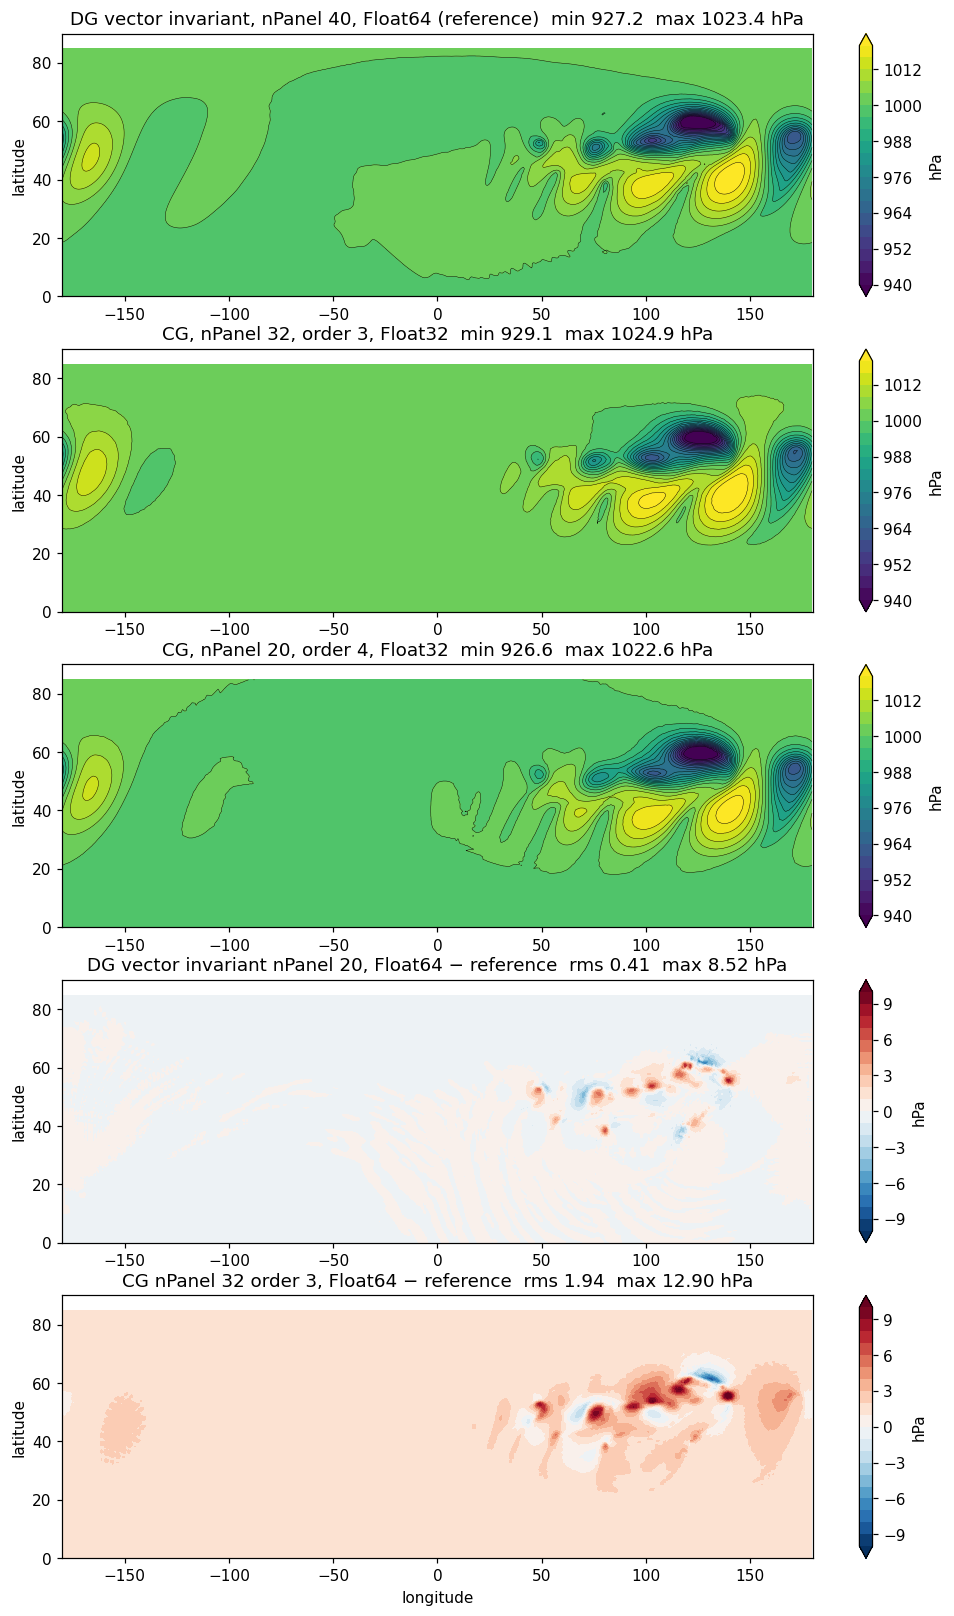
\includegraphics[height=0.8\textheight,keepaspectratio]{BaroWave10Days_ps.png}
\caption{Day-10 surface pressure: DGSEM VI reference ($n_\text{Panel}=40$),
CGSEM standard (order 3, $n_\text{Panel}=32$, shallow) and CG-A (order 4,
$n_\text{Panel}=20$) in Float32, and the Float64 differences of DGSEM VI
and CGSEM standard against the reference.}
\label{fig:all}
\end{figure}

\begin{figure}[p]
\centering
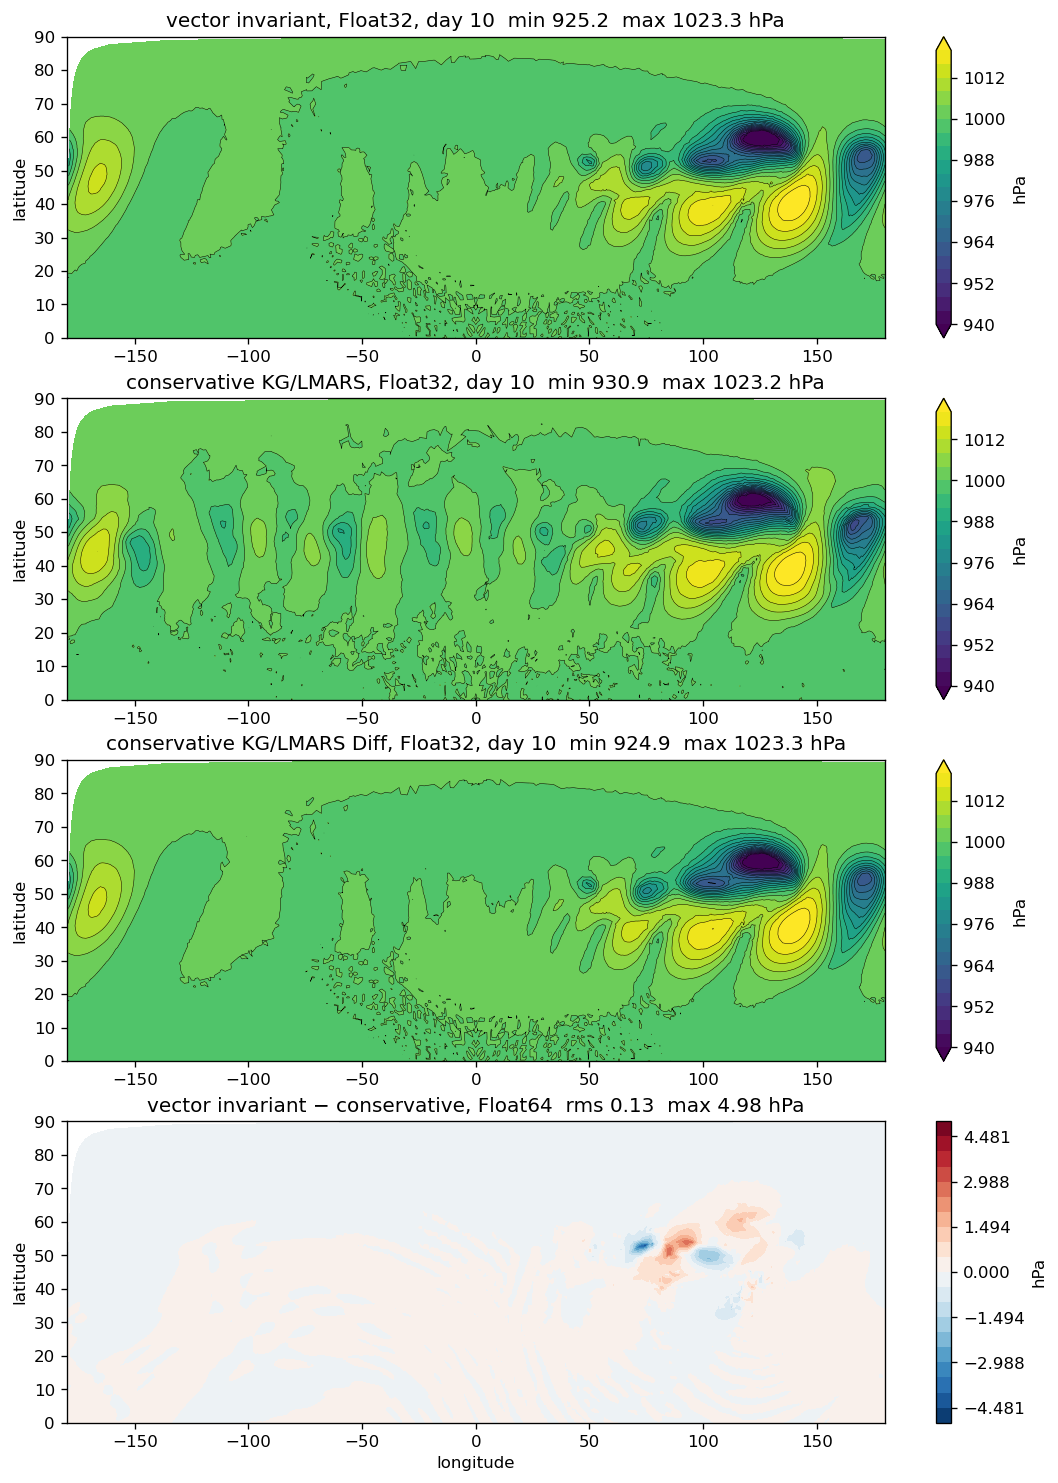
\includegraphics[width=0.92\textwidth]{BaroWave10Days_DG.png}
\caption{Day-10 surface pressure of the three DGSEM flux pairs in
Float32 ($n_\text{Panel}=20$, $N=4$) and the Float64 difference VI minus
Cons. The conservative fluxes with the full pressure develop spurious
waves in Float32.}
\label{fig:dg}
\end{figure}

\section*{Reproduction}

The scripts are in \code{bench/} of the Levante checkout. \code{bw10.jl}
(DGSEM) and \code{cgbw10.jl} (CGSEM) take the arguments of a job file
followed by overrides, run ten days without output and print the timing,
and they write the surface pressure. \code{cmp10.sh}, \code{cmp10cg.sh} and
\code{cmp10std.sh} are the batch scripts, and \code{cmp10\_all.py} produces
the tables and Figure~\ref{fig:all}.

\end{document}
